% ============================================================================
%  Mid-term presentation  (MPhil/MSc, Centre for Scientific Computing)
%  Effect of Floating-Point Precision and Hardware on HRSC Schemes
%  Author: Yudong Tang   Supervisor: Dr. Philip Blakely   Date: 05.06.2026
%  Built on BeamerMPhilTemplate.tex.  Compile: latexmk -pdf talk.tex
%
%  Deck is intentionally fuller than the 10-min spoken path.
%  [SPEAK]  = covered in the 10-minute talk
%  [BRIEF]  = shown, mentioned in one line, or skipped for time
% ============================================================================
\documentclass[xcolor=table]{beamer}
\usetheme{Madrid}
\usepackage{amssymb}
\usepackage{epsfig}
\usepackage{psfrag}
\usepackage{wrapfig}
\usepackage{graphicx}
\usepackage{color}
\usepackage{amsmath}
\usepackage{multimedia}
\usepackage{verbatim}
\usepackage{listings}
\usepackage{multicol}
\usepackage[table]{xcolor}
\usepackage{booktabs}
\usepackage{tikz}
\usetikzlibrary{arrows}

% Figures and banner images live in figs/
\graphicspath{{figs/}}

\DeclareSymbolFont{nosets}{U}{msb}{m}{7}
\DeclareMathSymbol{\natural}{\mathalpha}{nosets}{'116}
\DeclareMathSymbol{\real}{\mathalpha}{nosets}{'122}
\DeclareMathSymbol{\complex}{\mathalpha}{nosets}{'103}
\DeclareMathSymbol{\integer}{\mathalpha}{nosets}{'132}
\newcommand{\cross}{\wedge}
\newcommand{\vecdiv}{\nabla \cdot}
\newcommand{\grad}{\nabla}
\newcommand{\curl}{\nabla \cross}
\newcommand{\ifff}{\Leftrightarrow}
\newcommand{\sgn}{\text{sgn}}
\newcommand{\vect}[1]{\mathbf{#1}}
\newcommand{\sectref}[1]{\S\ref{#1}}
\providecommand{\norm}[1]{\lVert#1\rVert}
\usefonttheme{professionalfonts}

\lstset{language=C++}
\lstset{otherkeywords={<<<,>>>}}
\lstset{morekeywords={dim3,__host__,__kernel__,__global__,__device__}}
\lstset{breaklines,breakatwhitespace,breakautoindent=false,showstringspaces=false}
\lstset{keywordstyle=\color{purple}}
\lstset{identifierstyle=\color{blue}}
\lstset{basicstyle=\fontfamily{pcr}\fontsize{8pt}{8pt}\selectfont}
\lstset{linewidth=4.9in,xleftmargin=10pt}

\definecolor{lightblue}{rgb}{0.0,0.45,0.81}
\definecolor{lighterblue}{rgb}{0.415,0.678,0.894}
\definecolor{darkblue}{rgb}{0,0.243,0.447}
\definecolor{lightgreen}{rgb}{0,0.738,0.714}
\setbeamercolor{frametitle}{bg=lightgreen,fg=black}
\setbeamerfont{normal text}{family=arial}
\setbeamerfont{local structure}{family=arial}

\setbeamercolor*{author in head/foot}{bg=darkblue,fg=black}
\setbeamercolor*{logo in head/foot}{bg=white,fg=black}
\setbeamercolor*{title in head/foot}{bg=white,fg=black}
\setbeamercolor*{date in head/foot}{bg=white,fg=black}
\setbeamercolor{title}{bg=darkblue,fg=black}
\setbeamercolor{under headline}{bg=lighterblue}
\setbeamercolor{footline}{bg=darkblue}
\setbeamercolor{itemize item}{fg=black}
\setbeamercolor{item}{fg=black}
\setbeamerfont*{title in head/foot}{size=\small}
\setbeamerfont*{date in head/foot}{size=\small}
\setbeamertemplate{navigation symbols}{}
\defbeamertemplate*{title page}{customized}[1][]
{%
\usebeamerfont{subtitle}%
\usebeamercolor[fg]{subtitle}%
\begin{columns}[T]
  \begin{column}{0.4\paperwidth}
    \vspace{-0.05\paperheight}
\begin{beamercolorbox}[sep=1em,wd=0.37\paperwidth,ht=0.8\paperheight,left]{postit}%
\begin{centering}
  
\includegraphics[width=0.38\paperwidth]{UoC_Presentation_Cav_Banner_Image.png}
\end{centering}\\[0.15\paperheight]
\usebeamerfont{title}{\huge\inserttitle}
\usebeamerfont{subtitle}{\insertsubtitle}
{\flushright
\setbeamercolor{author}{bg=black,fg=Red}
\usebeamerfont{author} \insertauthor\\
\usebeamerfont{institute}\insertinstitute\\
\usebeamerfont{institute}Supervisor: Dr.~Philip Blakely\\
 }
\end{beamercolorbox}
\end{column}%
\begin{column}{0.55\paperwidth}%

\includegraphics[height=\paperheight]{UoC_Presentation_Title_Image.png}%
\end{column}%
\end{columns}%
\setbeamercolor{postit}{fg=black,bg=lightblue}%
}

\setbeamertemplate{frametitle}
{
  \begin{beamercolorbox}[wd=\paperwidth,ht=0.8cm,center]{logo in head/foot}%
  \usebeamerfont{logo in head/foot}
    
\includegraphics[width=\paperwidth]{UoC_Presentation_Full_Banner.png}
  \end{beamercolorbox}%
  \nointerlineskip%
  \begin{beamercolorbox}[wd=\paperwidth,ht=2.4ex,dp=0.8ex,leftskip=0.3cm]{frametitle}%
    \usebeamerfont{frametitle}\insertframetitle%
  \end{beamercolorbox}%
}

\setbeamertemplate{footline}
{
  \ifnum \theframenumber=1
    \else
    \leavevmode%
  \hbox{%
  \begin{beamercolorbox}[wd=.93\paperwidth,ht=0.8cm,left,dp=1ex]{logo in head/foot}%
\insertslidenavigationsymbol
\insertframenavigationsymbol
\insertsectionnavigationsymbol
\insertdocnavigationsymbol
\insertbackfindforwardnavigationsymbol
\vspace{0.2cm}
\end{beamercolorbox}%
\begin{beamercolorbox}[wd=0.07\paperwidth,ht=0.8cm,dp=1ex,right]{date in head/foot}%
    \insertframenumber{} / \inserttotalframenumber\hspace*{2ex}\vspace{0.2cm}
  \end{beamercolorbox}}%
  \vskip0pt%
\fi
}

% ----------------------------------------------------------------------------
\title[FP Precision \& Hardware in HRSC]{Effect of Floating-Point Precision and Hardware on HRSC Schemes}
\author{Yudong Tang}
\institute[CSC]{Centre for Scientific Computing, University of Cambridge}
\date{05.06.2026}

\begin{document}

% ===== Frame 1 : Title ====================================================
\begin{frame}
  \titlepage
\end{frame}

% ===== Frame 2 : Background / motivation =========================== [SPEAK]
\begin{frame}{Why precision and hardware matter}
\begin{itemize}
\item GPUs run \textbf{single precision} much faster than double, so there is a
      strong pull to drop precision in CFD codes to save time and memory.
\item But floating-point arithmetic is \textbf{not associative}: the same
      published algorithm, on a different device, compiler, or thread order,
      can give different bits.
\item In shock-capturing schemes those small differences can land exactly where
      the solution is most sensitive --- at shocks and contacts.
\end{itemize}
\vspace{0.4em}
\begin{block}{The question}
When we change precision or hardware, does the answer move --- by how much, and
\emph{where}?
\end{block}
\vspace{0.2em}
\footnotesize Plan: first confirm the solver is correct, then vary precision,
device, and compiler one at a time.
\note{
Good morning. My project is about how floating-point precision and hardware affect
high-resolution shock-capturing schemes -- the finite-volume methods we use for
compressible flow.

GPUs are much faster in single precision than in double, so there is a strong
reason to use single precision in CFD codes. But this is only safe if we know how
much accuracy we lose. There is also a second problem: floating-point addition is
not associative, so the same algorithm, built with a different compiler or run on
different hardware, can give slightly different numbers. In a code with shocks,
these differences can appear exactly where the solution is most sensitive. So my
main question is: when we change the precision or the hardware, does the answer
change, by how much, and where? In particular, does the same algorithm give the
same bits on a CPU and a GPU, and if not, why?
}
\end{frame}

% ===== Frame 3 : Numerical method (one text slide) ================ [SPEAK]
\begin{frame}{Numerical method}
\begin{columns}[T]
\begin{column}{0.52\textwidth}
\textbf{2D compressible Euler:} $U_t+F(U)_x+G(U)_y=0$,
$U=(\rho,\rho u,\rho v,E)^T$, with
{\scriptsize
\begin{equation*}
  F=\begin{pmatrix}\rho u\\ \rho u^2{+}p\\ \rho uv\\ u(E{+}p)\end{pmatrix},\ \
  G=\begin{pmatrix}\rho v\\ \rho uv\\ \rho v^2{+}p\\ v(E{+}p)\end{pmatrix}.
\end{equation*}}
\textbf{Interface flux $\widehat F$ chosen by the sign of the wave speeds:}
{\scriptsize
\begin{equation*}
  \widehat F_{\mathrm{HLLC}}=
  \begin{cases}
   F_L, & S_L\ge 0,\\
   F_{\ast L}, & S_L<0\le S_\ast,\\
   F_{\ast R}, & S_\ast<0\le S_R,\\
   F_R, & S_R<0.
  \end{cases}
\end{equation*}}
\end{column}
\begin{column}{0.46\textwidth}
\begin{itemize}
\item \textbf{MUSCL--Hancock} (2nd order): piecewise-linear reconstruction,
      \textbf{minmod} limiter, Hancock half-step.
\item \textbf{HLLC}: three waves $S_L,S_\ast,S_R$; restores the contact wave.
\item \textbf{Rusanov}: diffusive comparator, no contact branch.
\item Explicit step from a CFL limit on $|u|+c,\ |v|+c$.
\end{itemize}
\end{column}
\end{columns}
\note{
The system is the two-dimensional Euler equations. I solve them with a
finite-volume MUSCL--Hancock method, which is second order, with a minmod limiter
to control oscillations near shocks. At each cell face I use the HLLC Riemann
solver, which keeps the contact wave and chooses its flux from the sign of the
wave speeds. I also keep Rusanov, a more diffusive solver, only for comparison.
The time step comes from a CFL condition on the wave speeds. The important point
for later is this flux choice -- which side of the fan a cell is on -- because
that is where precision can change the result.
}
\end{frame}

% ===== Frame 4 : Floating-point details + how tested ============== [SPEAK]
\begin{frame}[shrink=18]{Floating-point details, and how it is tested}
\begin{columns}[T]
\begin{column}{0.5\textwidth}
\textbf{Where precision enters}
\begin{itemize}
\item Every operation is rounded; FMA and fast-math change the last bits.
\item Pressure recovery $p=(\gamma-1)\big(E-\tfrac12\rho|\mathbf u|^2\big)$
      loses digits when kinetic energy nears total energy --- this feeds the
      wave speeds.
\item HLLC branch ($<$ vs $\le$) matters only when a wave speed $\approx 0$,
      where the contact speed $S_\ast$ is a division (full form below).
\end{itemize}
\end{column}
\begin{column}{0.48\textwidth}
\textbf{How it is tested}
\begin{itemize}
\item One code base; vary precision (fp32/fp64), device (CPU/GPU), build
      (\texttt{STRICT\_IEEE} / \texttt{FAST\_MATH}).
\item Metrics: $L_1$, $L_\infty$, ULP (bits).
\item References: exact Riemann (1D), high-res fp64 (2D).
\item Hardware: local i9 / RTX~4060; CSC EPYC / RTX~5090.
\end{itemize}
\end{column}
\end{columns}
\vspace{0.1em}
{\scriptsize
\begin{equation*}
  S_\ast=\frac{N_\ast}{D_\ast},\quad
  N_\ast=(p_R-p_L)+\rho_L u_L(S_L-u_L)-\rho_R u_R(S_R-u_R),\quad
  D_\ast=\rho_L(S_L-u_L)-\rho_R(S_R-u_R),
\end{equation*}
\vspace{-0.8em}
\begin{equation*}
  S_L=\min(u_L-a_L,u_R-a_R),\qquad S_R=\max(u_L+a_L,u_R+a_R).
\end{equation*}}
\centering{\footnotesize Near-vacuum: $N_\ast$ cancels to $0$ --- an $S_\ast{=}0$
tie the dispatcher must handle (implementation detail, not instability).}
\note{
There are three places where precision can enter. First, every operation is
rounded. Second, the pressure is computed by subtracting kinetic energy from total
energy; when these are close, the subtraction loses accuracy, and this error goes
into the sound speed and the wave speeds. Third, the HLLC branch test only matters
when a wave speed is very close to zero, because the contact speed is a division.
I study this with one code base, changing only one thing at a time -- precision,
device, or build flags. I measure the difference three ways: the L-one norm for
overall size, L-infinity for the worst cell, and ULP, meaning how many bits
differ. My references are the exact Riemann solution in 1D and a high-resolution
double-precision run in 2D.
}
\end{frame}

% ===== Frame 6 : Validation 1D (Sod) ============================= [SPEAK]
\begin{frame}{Validation: 1D shock tubes}
\begin{itemize}
\item Sod and the Toro tests sit on the exact Riemann solution, with the expected
      smearing over a few cells at the discontinuities.
\item This fixes the discretisation-error scale that the precision differences
      are later compared against.
\end{itemize}
\vspace{0.1em}
\centering

\includegraphics[width=0.88\textwidth]{sod_comparison}\\[0.2em]
\footnotesize Sod, $N=200$, $t=0.25$: MUSCL--Hancock--HLLC vs the exact Riemann
solution (density, velocity, pressure).
\note{
Before looking at any precision difference, I show the solver is correct. In one
dimension, Sod and the Toro tests match the exact Riemann solution, with the usual
smearing over a few cells at the discontinuities. This slide mainly fixes the
scale: the discretisation error of the method is what I later compare the precision
differences against.
}
\end{frame}

% ===== Frame 6 : Validation 2D (LW3) ============================= [SPEAK]
\begin{frame}{Validation: 2D Riemann problem}
\begin{itemize}
\item Liska--Wendroff structures are reproduced; the error against the
      high-resolution fp64 reference drops with refinement.
\item From here on, any difference shown is a precision or hardware effect ---
      not a bug.
\end{itemize}
\vspace{0.1em}
\centering

\includegraphics[width=0.9\textwidth]{lw3_n400_comparison}\\[0.2em]
\footnotesize Liska--Wendroff configuration~3 at $400^2$: reference (left)
vs.\ this work (right).
\note{
In two dimensions, the Liska--Wendroff tests reproduce the published shock and
contact structures, and the error against the high-resolution reference goes down
as I refine the grid. My result is on the right, the reference on the left. From
here on, any difference I show is a precision or hardware effect, not a bug.
}
\end{frame}

% ===== Frame 8 : Finding 1 --- single vs double ================== [SPEAK]
\begin{frame}{Finding 1: single vs double precision}
\begin{itemize}
\item The direct fp32$-$fp64 difference stays $\sim$5 decades below the
      discretisation error --- single precision is \emph{adequate} here.
\item But it is not uniform: it concentrates on shock fronts and contacts
      (largest density ratio $R_\rho\lesssim 1.3\times10^{-4}$).
\end{itemize}
\vspace{0.1em}
\centering

\includegraphics[width=0.86\textwidth]{fp32_fp64_density_differences_2d_pair}\\[0.2em]
\footnotesize $|\rho_{\mathrm{fp32}}-\rho_{\mathrm{fp64}}|$ for LW3 (left) and
LW12 (right) at $400^2$ --- noise rides the wave structure, near zero elsewhere.
\note{
Now the first result. Comparing single and double precision directly, the
difference stays about five orders of magnitude below the discretisation error. I
see this clearly in the 1D cases, where the precision noise is far below the
exact-solution error at the same shocks and contacts. This means single precision
is good enough here -- it does not change the results we report. But the difference
is not uniform. This 2D map shows where it is, with density contours on top: it
sits on the shock fronts and contacts, and is almost zero in the smooth regions.
One point to be careful about: this ratio grows a little with resolution, because
the reference error shrinks faster than the precision difference. So single
precision is fine away from the fronts, and the fronts are where it concentrates.
}
\end{frame}

% ===== Frame 9 : Finding 2 --- CPU vs GPU + compiler ============= [SPEAK]
\begin{frame}{Finding 2: CPU vs GPU, and what breaks the match}
\small
\begin{itemize}
\setlength\itemsep{0.15em}
\item Matched strict-IEEE HLLC: CPU vs GPU is \textbf{bit-identical} ---
      $L_1=L_\infty=\mathrm{ULP}_{\max}=0$, all five cases (final + checkpoints).
\item Conditional: fast-math breaks it (ULP $\approx 30$) and the gap
      \emph{grows in time} --- reproducibility is a property of the
      \textbf{build}, not the hardware.
\end{itemize}
\vspace{-0.2em}
\centering

\includegraphics[height=0.46\textheight,width=0.72\textwidth,keepaspectratio]{drift_timeseries_l1_native}\\[-0.1em]
{\scriptsize \textbf{O2 strict-IEEE vs Ofast+fast-math drift} (1D); matched strict
CPU/GPU $=0$.}
\note{
The second result is about hardware. With the matched strict-IEEE build -- that
is, with fast-math off -- the same case on CPU and GPU is bit-for-bit identical:
zero in all three metrics, for all five cases, on final outputs and saved
checkpoints, including a run on the CSC cluster. With controlled flags, the GPU is
not the source of the difference. The optimisation level alone also does not
matter: O2 and O3 gave identical bits. But this depends on the build. If I turn
fast-math back on, the results change by up to about thirty ULP, and this plot
shows that difference growing in time, not staying fixed. Reproducibility here
depends on the build flags, not the hardware: same algorithm, same machine,
different flags, different answer.
}
\end{frame}

% ===== Frame 9 : Solver sensitivity --- HLLC vs Rusanov ========== [SPEAK]
\begin{frame}{How big are these effects? Solver vs the rest}
\begin{itemize}
\item Changing the Riemann solver (HLLC $\to$ Rusanov) is by far the largest
      effect --- but it is a \emph{method} change, not reproducibility drift.
\end{itemize}
\begin{center}
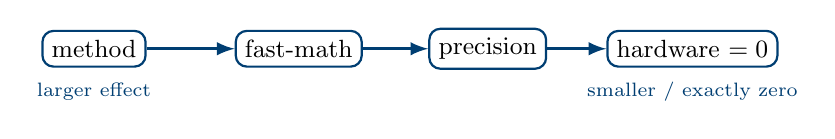
\begin{tikzpicture}[>=latex,every node/.style={font=\small}]
 \node[draw=darkblue,thick,rounded corners] (m) at (0,0)   {method};
 \node[draw=darkblue,thick,rounded corners] (f) at (2.6,0) {fast-math};
 \node[draw=darkblue,thick,rounded corners] (p) at (5.0,0) {precision};
 \node[draw=darkblue,thick,rounded corners] (h) at (7.6,0) {hardware $=0$};
 \draw[->,very thick,darkblue] (m)--(f);
 \draw[->,very thick,darkblue] (f)--(p);
 \draw[->,very thick,darkblue] (p)--(h);
 \node[font=\scriptsize,darkblue] at (0,-0.55)   {larger effect};
 \node[font=\scriptsize,darkblue] at (7.6,-0.55) {smaller / exactly zero};
\end{tikzpicture}
\end{center}
\vspace{0.1em}
\centering

\includegraphics[width=0.8\textwidth]{density_hllc_vs_rusanov_200}\\[0.2em]
\footnotesize LW3 $200^2$ density, HLLC vs Rusanov at $t=0.3$, \textbf{CFL $=0.5$}:
a visible, method-level difference --- the scale reference for the smaller precision and
hardware effects.
\note{
It helps to put these effects on one scale. The biggest change I can make without
changing the mathematics is the Riemann solver itself: replacing HLLC with the
more diffusive Rusanov gives a clearly visible difference, shown here. But this is
a method change, not reproducibility drift. It sets the order for everything else:
the method difference is large; fast-math is much smaller; single-versus-double is
smaller still; and the matched CPU-versus-GPU difference is exactly zero. What
really threatens reproducibility is the implementation and the build choices, in
that order, not the device.
}
\end{frame}

% ===== Frame 10 : Verificarlo overview ========================== [SPEAK]
\begin{frame}{Verificarlo: Monte-Carlo arithmetic}
\small
Verificarlo re-runs the solver with randomly-rounded arithmetic at a chosen
\emph{virtual} precision (\texttt{p8}/\texttt{p16}/\texttt{p32} mantissa bits),
$n=30$ seeds. The ensemble spread relative to the reference error
$\eta=\sigma_{\mathrm{FP}}/|\rho-\rho_{\mathrm{ref}}|$ (log scale) shows where
rounding dominates --- red ($\eta>1$) is precision-limited.

\vspace{0.4em}
\centering

\includegraphics[width=0.84\textwidth]{noise_to_error_ratio_heatmap_grid_rho}

{\footnotesize LW3 density (HLLC): $\eta$ across \texttt{p8}, \texttt{p16},
\texttt{p32}.}
\note{
Verificarlo works by replacing every floating-point operation with a randomly
rounded version -- Monte-Carlo arithmetic -- and I run the case thirty times, so
the spread across the ensemble tells me how uncertain each cell is to rounding.
The virtual precision, p8, p16 or p32, just sets how many mantissa bits are kept,
so it is a what-if precision independent of how the code was actually built. The
diagnostic I plot is the ratio of that rounding spread to the reference error, on
a log scale: where log eta is greater than zero, the rounding noise is larger than
the discretisation error, so that cell is precision-limited.
}
\end{frame}

% ===== Frame 11 : Where precision bites --- Verificarlo ========== [SPEAK]
\begin{frame}{Where precision bites: virtual-precision diagnostics}
\begin{itemize}
\item Verificarlo injects rounding at a chosen \emph{virtual} precision and runs
      a 30-seed ensemble --- locating sensitivity without changing hardware.
\item Precision-limited fraction
      ($\eta=\sigma_{\mathrm{FP}}/|U_{\mathrm{fp64}}-U_{\mathrm{ref}}|>1$) shrinks
      with precision and reaches $0\%$ at \texttt{p32}; the shock fronts clear
      last.
\end{itemize}
\vspace{0.1em}
\centering

\includegraphics[width=0.82\textwidth]{region_noise_to_error_ratio_precision_grid_rho}\\[0.2em]
\footnotesize LW3 density (HLLC): noise-to-error ratio by region at \texttt{p8},
\texttt{p16}, \texttt{p32}.
\note{
This is the result, split by region. As I raise the virtual precision, the
fraction of precision-limited cells falls: at p8 most of the field is
precision-limited, and by the single-precision level it reaches zero in every
region. The last region to clear is the shock front -- the same story the direct
single-versus-double comparison told. So Verificarlo locates the sensitivity
rather than just bounding it, and it points at the fronts.
}
\end{frame}

% ===== Frame 10 : Conclusions + Report 2 ========================= [SPEAK]
{
\setbeamertemplate{background}
{
\includegraphics[width=\paperwidth,height=\paperheight]{UoC_Full_Slide_Background.png}}
\begin{frame}{Conclusions and Report 2}
\begin{itemize}
\item Single precision is adequate for these Euler cases, but its error
      concentrates on shock fronts.
\item CPU and GPU agree to the bit under strict-IEEE --- irreproducibility comes
      from build flags and solver detail, not the device.
\item Largest effects: the Riemann solver (a method change) and fast-math; the
      branch rule ($<$ vs $\le$) is only roundoff after fixing an $S_\ast{=}0$ tie
      (an implementation detail, not instability).
\item Verificarlo (virtual precision) locates the sensitivity: the
      precision-limited area shrinks as precision rises and is essentially gone by
      single precision, with the shock fronts the last to clear.
\item \textbf{Report 2:} extend the time-resolved drift framework to ideal-MHD,
      with divergence cleaning and long-time (chaotic) separation.
\end{itemize}
\vspace{0.4em}
\centering\footnotesize Thank you --- questions welcome.
\note{
To summarise. Single precision is good enough for these Euler cases, but its error
concentrates at the fronts. CPU and GPU agree to the bit under strict-IEEE, so the
irreproducibility people worry about comes from the build flags and the solver
detail, not the device -- the Riemann solver and fast-math were the largest
effects. The strict versus non-strict branch rule turned out to be only roundoff
once I fixed an implementation tie-case at zero wave speed, so it is an
implementation detail, not instability. Verificarlo, using virtual precision, then
locates where precision
matters: the precision-limited area shrinks as precision rises and is essentially
gone by single precision, with the shock fronts the last to clear. For Report 2,
I will take the same drift-in-time method to ideal-MHD,
where divergence cleaning and chaotic behaviour make the long-time behaviour the
interesting question. Thank you -- I am happy to take questions.
}
\end{frame}
}

% ========================== BACKUP SLIDES ==========================
\begin{frame}[plain]
\centering\vfill
{\Large\bfseries Backup slides}\\[0.3em]
\footnotesize for questions
\vfill
\end{frame}

\begin{frame}{Backup: HLLC interface wave fan}
\centering {\small\itshape Supplements slide~3 (Numerical method) --- HLLC wave structure behind the flux-branch choice.}\\[0.4em]

\includegraphics[height=0.60\textheight]{ch3_hllc_fan}\\[0.2em]
\footnotesize $S_L,S_\ast,S_R$ separate $U_L,U_{\ast L},U_{\ast R},U_R$; the flux
branch is selected by the sign of these three wave speeds.
\end{frame}

\begin{frame}{Backup: 1D strong-shock validation (Toro3)}
\centering {\small\itshape Supplements slide~5 (Validation 1D) --- a strong-shock Toro test beyond Sod.}\\[0.4em]

\includegraphics[width=0.82\textwidth]{toro3_comparison}\\[0.2em]
\footnotesize Toro3, $N=200$: a right-running supersonic shock vs the exact
Riemann solution (Toro5 behaves similarly).
\end{frame}

\begin{frame}{Backup: 2D validation --- LW12}
\centering {\small\itshape Supplements slide~6 (Validation 2D) --- the second 2D Riemann case.}\\[0.4em]

\includegraphics[width=0.92\textwidth]{lw12_n400_comparison}\\[0.2em]
\footnotesize Liska--Wendroff configuration~12 at $400^2$: reference (left)
vs.\ this work (right).
\end{frame}

\begin{frame}{Backup: fp32$-$fp64 noise vs discretisation error (1D)}
\centering {\small\itshape Supplements slide~7 (single vs double) --- the gap quantified against discretisation error.}\\[0.4em]

\includegraphics[width=\textwidth]{fp32_fp64_density_differences_1d_triplet}\\[0.2em]
\footnotesize Sod/Toro3/Toro5: cellwise $\rho_{\mathrm{fp32}}-\rho_{\mathrm{fp64}}$
(top) sits $\sim$5 decades below the fp64$-$exact error (bottom).
\end{frame}

\begin{frame}{Backup: implementation \& experiment pipeline}
\centering {\small\itshape Supplements slide~4 (how it is tested) --- one binary, one axis changed at a time.}\\[0.4em]

\includegraphics[height=0.64\textheight]{ch4_architecture_workflow}\\[0.2em]
\footnotesize Stand-alone CPU/CUDA code: setup, time-stepping execution, analysis
(saved states, metrics).
\end{frame}

\begin{frame}{Backup: branch-rule audit (corrected)}
\centering {\small\itshape Supplements slides~4 \& 12 --- the $<$ vs $\le$ branch rule after fixing the $S_\ast{=}0$ tie.}\\[0.4em]
\small
\begin{tabular}{@{}lrrr@{}}
\toprule
Case & $L_1$ & $L_\infty$ & $\mathrm{ULP}_{\max}$ \\
\midrule
Sod                   & 0        & 0        & 0    \\
Stationary contact    & 0        & 0        & 0    \\
Toro2                 & 2.96e-16 & 4.00e-15 & 6.0  \\
Toro3 / Toro4 / Toro5 & 0        & 0        & 0    \\
LW3 $200^2$           & 4.97e-16 & 1.44e-14 & 15.1 \\
\bottomrule
\end{tabular}\\[0.4em]
\footnotesize After fixing an implementation tie-case at $S_\ast{=}0$, all strict
runs complete and $\le$ vs $<$ differs only at roundoff scale --- no failure. The
earlier Toro-2 ``strict failure'' was that defect, not strict-HLLC instability.
Strict-HLLC CPU/GPU validation (LW3 $200^2$/$400^2$, fp64) stays $0/0/0$.
\end{frame}

\begin{frame}{Backup: MCA roundoff scale vs precision}
\centering {\small\itshape Supplements slides~11--12 (Verificarlo) --- how the rounding scale falls with precision.}\\[0.4em]

\includegraphics[width=0.66\textwidth]{sigma_fp_vs_precision}\\[0.2em]
\footnotesize MCA-estimated $\sigma_{\mathrm{FP}}$ for LW3 density falls with
virtual precision (HLLC blue, Rusanov grey).
\end{frame}

\begin{frame}{Backup: LoSoS region margin at \texttt{p32}}
\centering {\small\itshape Supplements slides~11--12 (Verificarlo) --- significant digits available vs required, by region.}\\[0.4em]

\includegraphics[width=0.66\textwidth]{region_losos_margin_rho_p32}\\[0.2em]
\footnotesize Available significant digits minus the required threshold at
\texttt{p32}: positive in the smooth interior, negative on the shock front.
\end{frame}

\begin{frame}{Backup: ideal-MHD seven-wave fan (Report 2)}
\centering {\small\itshape Supplements slide~13 (Conclusions / Report 2) --- the MHD wave structure ahead.}\\[0.4em]

\includegraphics[width=0.9\textwidth]{ch3_mhd_seven_wave_fan}\\[0.2em]
\footnotesize Ideal-MHD adds two fast, two Alfv\'en, two slow waves and the
entropy mode --- the Report~2 system.
\end{frame}

% ============================ BACKUP: DATA TABLES ============================
\begin{frame}[plain]
\centering\vfill {\Large\bfseries Backup --- key data tables}\vfill
\end{frame}

\begin{frame}{Backup table: matched CPU/GPU strict-IEEE coverage}
\centering {\small\itshape Supplements slide~8 (CPU vs GPU) --- the full coverage behind ``0/0/0''.}\\[0.4em]
\small
\begin{tabular}{@{}lllc@{}}
\toprule
Case & Precision & Final / checkpoints & Drift \\
\midrule
Sod   & fp32, fp64 & 2 / 8 (to $t=0.25$)    & zero \\
Toro3 & fp32, fp64 & 2 / 4 (25/50/75/100\%) & zero \\
Toro5 & fp32, fp64 & 2 / 4 (25/50/75/100\%) & zero \\
LW3   & fp32, fp64 & 4 / 16 ($200^2,400^2$) & zero \\
LW12  & fp32, fp64 & 4 / 16 ($200^2,400^2$) & zero \\
\bottomrule
\end{tabular}\\[0.4em]
\footnotesize ``Zero'' $= L_1=L_\infty=\mathrm{ULP}_{\max}=0$ on saved
conservative states (final outputs + checkpoints).
\end{frame}

\begin{frame}{Backup table: sensitivity axes (CPU fp64)}
\centering {\small\itshape Supplements slides~8--9 (what breaks the match / hierarchy) --- the numbers.}\\[0.4em]
\small
\begin{tabular}{@{}llrr@{}}
\toprule
Comparison & evidence & $L_1$ & $L_\infty$ \\
\midrule
HLLC branch $\le$ vs $<$ & all cases (tie-fixed) & 4.97e-16 & 1.44e-14 \\
O2 vs O3                 & all tested           & 0        & 0 \\
O2 vs Ofast+fast-math    & Toro5 $N{=}200$      & 4.57e-13 & 7.41e-11 \\
HLLC vs Rusanov          & LW3 $200^2$          & 8.58e-3  & 1.45 \\
\bottomrule
\end{tabular}\\[0.4em]
\footnotesize Branch/optimisation at roundoff; fast-math dominates compiler
drift; HLLC--Rusanov is a method effect, not drift.
\end{frame}

\begin{frame}{Backup table: 2D density validation \& precision scale}
\centering {\small\itshape Supplements slides~6--7 (Validation 2D / single vs double) --- error and precision scale.}\\[0.4em]
\small
\begin{tabular}{@{}llrcrr@{}}
\toprule
Case & ref / grid & fp64 $L_1$ & SSIM & $R_\rho^{\mathrm{ref}}$ & $R_p^{\mathrm{ref}}$ \\
\midrule
LW3  & $1600^2$, $200^2$ & 7.89e-3 & 0.9663 & 4.47e-5 & 1.34e-5 \\
LW3  & $1600^2$, $400^2$ & 4.95e-3 & 0.9817 & 9.25e-5 & 2.59e-5 \\
LW12 & $800^2$, $200^2$  & 2.95e-3 & 0.9890 & 4.63e-5 & 3.85e-5 \\
LW12 & $800^2$, $400^2$  & 1.33e-3 & 0.9963 & 1.30e-4 & 1.13e-4 \\
\bottomrule
\end{tabular}\\[0.4em]
\footnotesize fp32--fp64 ratios stay $\lesssim 10^{-4}$ against the
high-resolution fp64 reference.
\end{frame}

% ============================== REFERENCES ==============================
\setbeamertemplate{bibliography item}{}
\begin{frame}[allowframebreaks]{References}
\tiny
\nocite{*}
\bibliographystyle{apalike}
\bibliography{references}
\end{frame}

\end{document}
